The structure of a possible instantiation of the toll system can be seen in the following composite structure diagrams. In this case an enterprise server is connected to a single toll station, which is connected to one lane of each type, creating a station that is both an entrance and an exit. Each lane communicates with the enterprise server via the station server.
\\
\begin{figure}[H]
\centerline{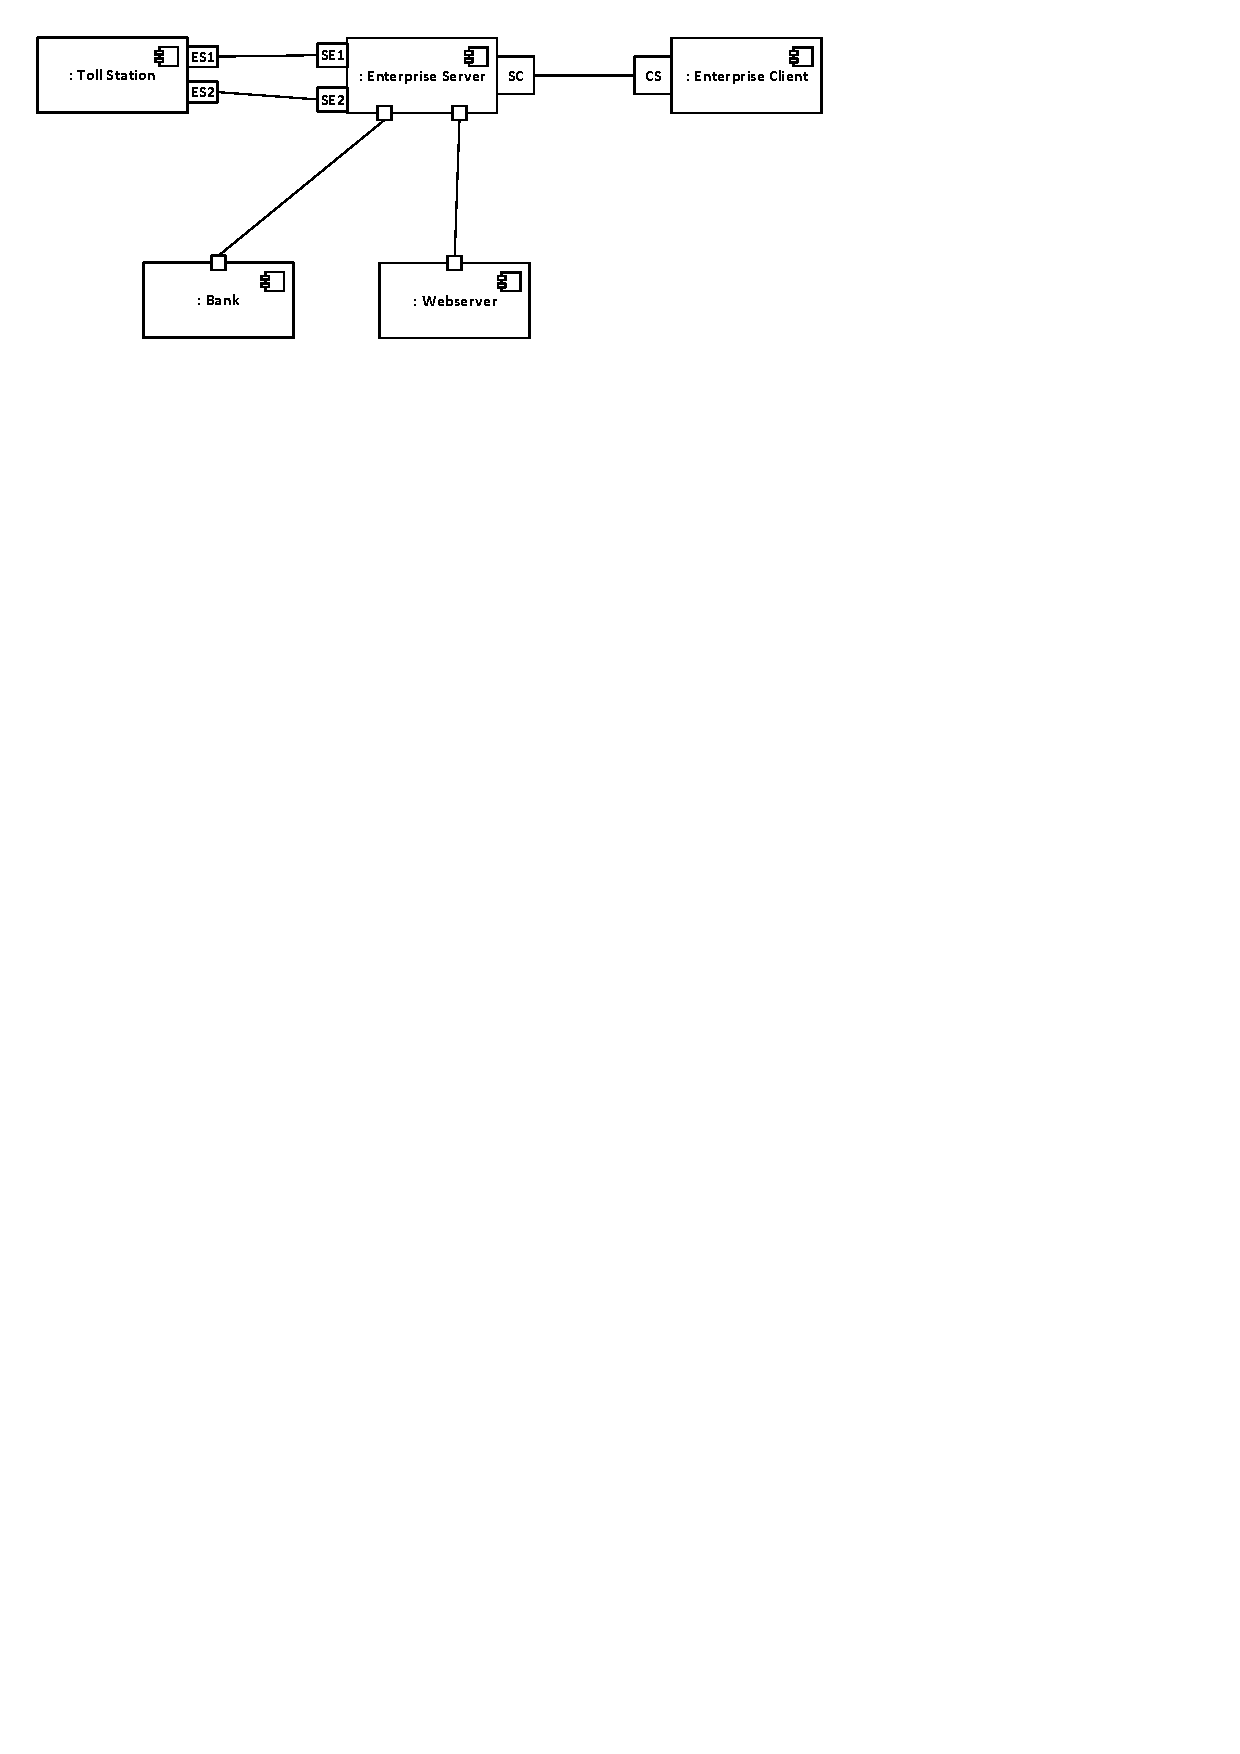
\includegraphics[width=\textwidth]{img/composite_structure_diagrams/cscd_enterprise}}
\caption{Composite structure diagram for the entire toll system}
\label{fig:csd_e}
\end{figure}

\begin{figure}[H]
\centerline{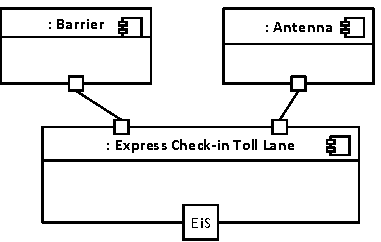
\includegraphics[width=\textwidth]{img/composite_structure_diagrams/cscd_toll_lane_express_in}}
\caption{The structure of the express check in lane}
\label{fig:csd_tlei}
\end{figure}

\begin{figure}[H]
\centerline{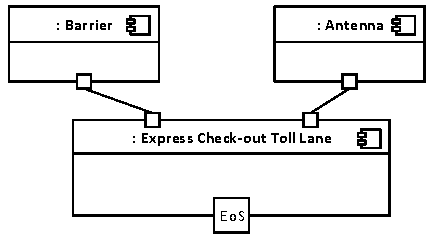
\includegraphics[width=\textwidth]{img/composite_structure_diagrams/cscd_toll_lane_express_out}}
\caption{The structure of the express check out lane}
\label{fig:csd_tleo}
\end{figure}

\begin{figure}[H]
\centerline{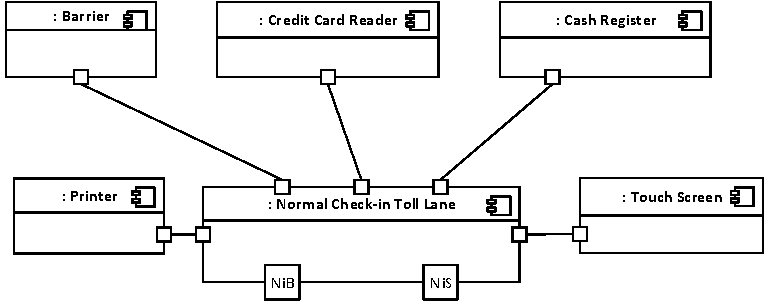
\includegraphics[width=\textwidth]{img/composite_structure_diagrams/cscd_toll_lane_normal_in}}
\caption{The structure of the normal check in lane}
\label{fig:csd_tlni}
\end{figure}

\begin{figure}[H]
\centerline{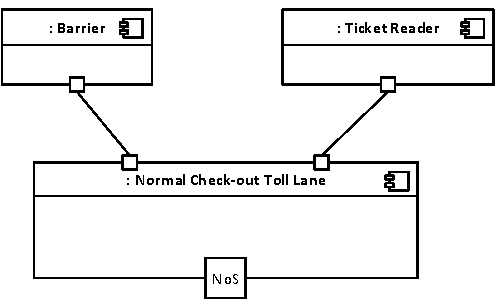
\includegraphics[width=\textwidth]{img/composite_structure_diagrams/cscd_toll_lane_normal_out}}
\caption{The structure of the normal check out lane}
\label{fig:csd_tlno}
\end{figure}


\begin{figure}[H]
\centerline{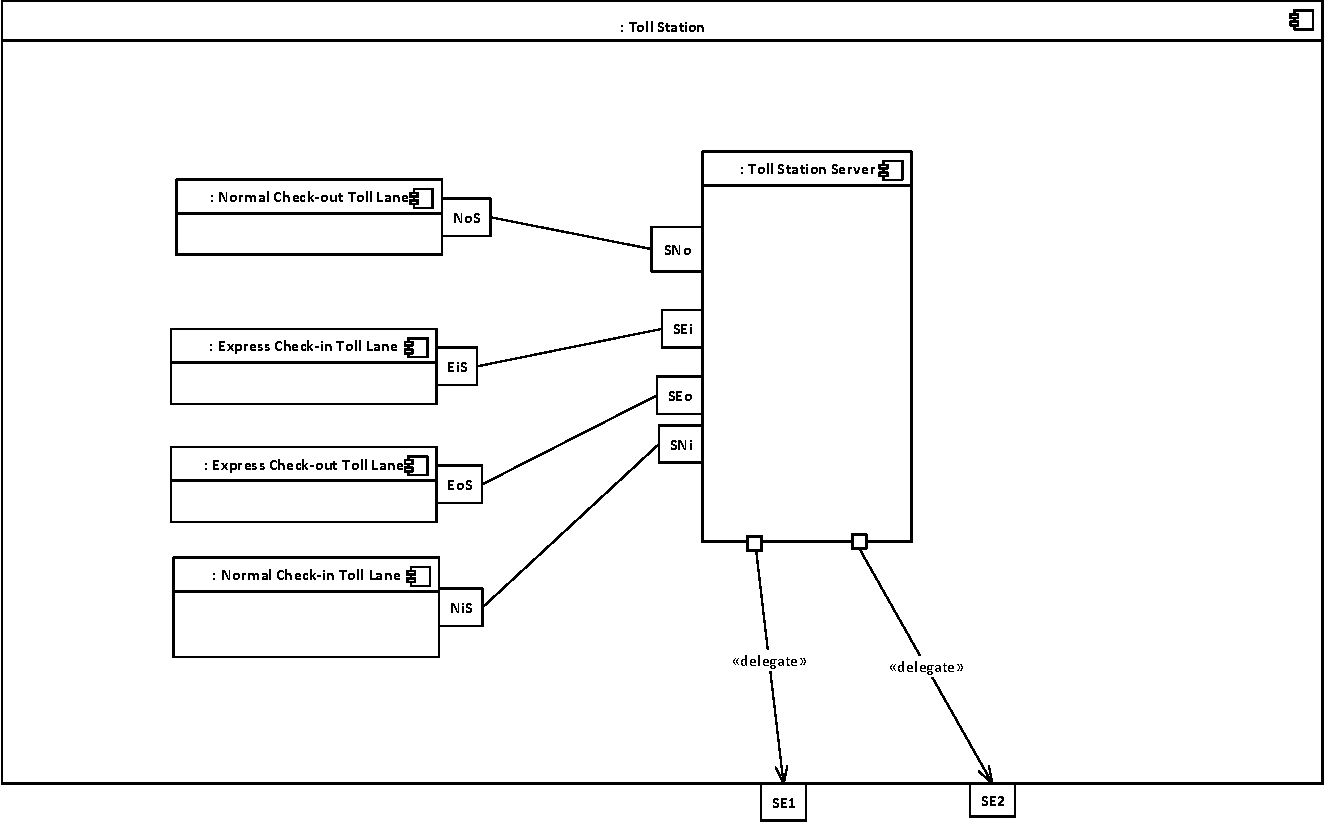
\includegraphics[width=\textwidth]{img/composite_structure_diagrams/cscd_toll_station}}
\caption{The structure of the toll station}
\label{fig:csd_ts}
\end{figure}
